\section{Loading parameters}
In addition to simply running kernels, the CPU may load parameters to the kernel, using the \verb/load_constant/ function.
Listing \ref{lst:load-constant} shows the process of setting kernel parameters.

\begin{c-code}[caption=Setting a kernel parameter, label=lst:load-constant]
load_constant(0, 0x07E0);
\end{c-code}

\begin{figure}[H]
    \centering
    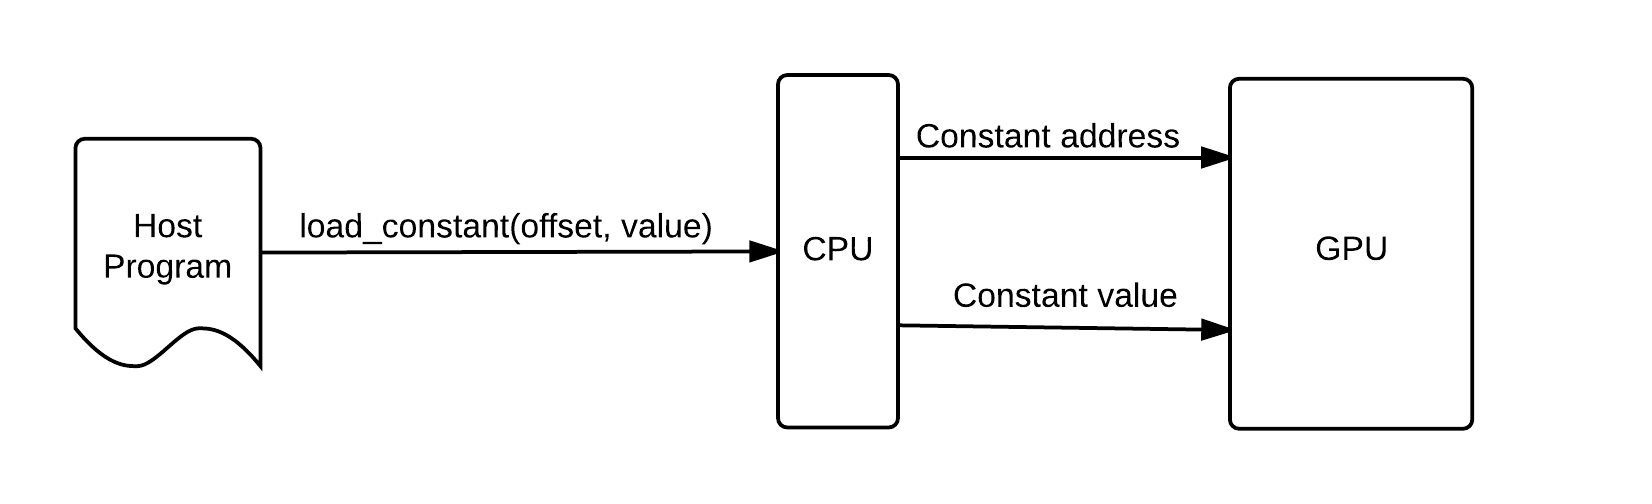
\includegraphics[width=\textwidth]{../cpu/diagrams/loading_a_constant.png}
    \caption{CPU-GPU interaction when loading a parameter.}
    \label{fig:loading_a_constant}
\end{figure}

Constants are written to the GPU in one chunk, as their size align with the size of the data bus.
As seen in figure \ref{fig:load_constant_format}, the constant memory has no offset in the FPGA address space.

\begin{figure}[H]
    \centering
    \begin{tabular}{|c|c|c|}
    \multicolumn{1}{c}{1} & \multicolumn{1}{c}{3} & \multicolumn{1}{c}{16} \\ \hline
    X & 000 & address \\ \hline
    \end{tabular}
    \caption{Address format for loading a parameter.}
    \label{fig:load_constant_format}
\end{figure}
